\chapter{Projeto do aplicativo}

  \section{Descrição do aplicativo}
    O \textit{BORAFUT} é um aplicativo móvel multiplataforma destinado à organização de partidas de futebol amador no Distrito Federal. Seu objetivo é centralizar informações que atualmente se encontram dispersas em conversas informais, reduzindo a dificuldade de marcar jogos, confirmar presença de jogadores e utilizar de forma eficiente as quadras públicas disponíveis.

    O aplicativo foi projetado com base nas dores identificadas durante a fase de observação e confirmadas pelos dados do questionário aplicado a mais de 70 praticantes de futebol amador. Os resultados indicaram que a organização de partidas ocorre predominantemente por meio de grupos de WhatsApp, com alta taxa de cancelamento de jogos, desencontros de informação e pouca visibilidade sobre quadras disponíveis. Esse cenário motivou a criação de uma solução que facilite a coordenação entre jogadores e torne o processo de organizar partidas mais simples e previsível.

    O público-alvo inicial do \textit{BORAFUT} é composto majoritariamente por jovens adultos entre 18 e 30 anos, praticantes amadores de futsal e \textit{society}, que jogam em quadras públicas e possuem grupos estabelecidos, mas dependem de comunicação manual e descentralizada. Esse grupo representa o perfil predominante identificado na pesquisa empírica e é o foco do MVP.

    A proposta de valor do \textit{BORAFUT} é oferecer uma plataforma única e organizada para gerenciar partidas de futebol amador, reduzindo o esforço de coordenação entre os jogadores e evitando problemas comuns como desencontros, falta de informação e cancelamentos. O aplicativo reúne, em um único ambiente, funcionalidades que hoje estão dispersas entre conversas informais, listas manuais e grupos de mensagem.

    As principais funcionalidades previstas para o MVP incluem:
    \begin{itemize}
        \item \textbf{visualização de quadras e locais de jogo próximos}, com base em geolocalização;
        \item \textbf{criação de partidas}, definindo horário e local;
        \item \textbf{confirmação de presença dos participantes} e acompanhamento em tempo real do número de participantes;
        \item \textbf{autenticação por código enviado por e-mail} (modelo passwordless), simplificando o ingresso no sistema;
        \item \textbf{exibição centralizada das informações essenciais da partida}, como horário, endereço e modalidade;
        \item \textbf{formação automática de times}, com base na ordem de chegada, facilitando o início do jogo e evitando conflitos.
    \end{itemize}  

    No escopo do MVP, o \textit{BORAFUT} prioriza funcionalidades essenciais para organizar jogos de forma simples e funcional, sem incluir recursos avançados que deverão fazer parte de versões futuras do sistema, caso sejam validados como relevantes pelos usuários.

  \section{Escopo do MVP}
    O MVP do \textit{BORAFUT} foi definido a partir das necessidades prioritárias identificadas durante a fase de elicitação e análise (Capítulo~\ref{sec:metodologia-elicitacao}). Seu objetivo é entregar uma solução funcional mínima que permita organizar partidas de futebol amador de forma simples, confiável e centralizada.

    Os requisitos foram definidos a partir das técnicas de elicitação e priorização apresentadas na Seção~\ref{sec:metodologia-elicitacao}. 

    Os requisitos foram organizados em duas categorias: Requisitos Funcionais (RF), que descrevem os comportamentos esperados do sistema, e Requisitos Não Funcionais (RNF), que estabelecem restrições técnicas e propriedades de qualidade. A seguir, são apresentados alguns dos requisitos mais representativos do MVP.

    \subsection{Requisitos funcionais}
      Os requisitos funcionais descrevem as ações que o sistema deve ser capaz de executar no escopo do MVP. Alguns exemplos incluem:

      \begin{itemize}
          \item \textbf{RF01 – Autenticação por e-mail:} o sistema deve permitir que usuários realizem login informando apenas o e-mail, recebendo um código temporário para acesso.
          
          \item \textbf{RF02 – Visualização de quadras:} o sistema deve exibir um mapa interativo com quadras públicas próximas ao usuário, permitindo navegação e pesquisa.

          \item \textbf{RF03 – Criação de partidas:} o sistema deve permitir que usuários registrem um fut, informando quadra, horário, modalidade e número de vagas.

          \item \textbf{RF04 – Confirmação de presença:} o sistema deve permitir que usuários confirmem presença em partidas abertas, exibindo em tempo real as vagas remanescentes.

          \item \textbf{RF05 – Formação automática de times:} o sistema deve gerar times com base na ordem de confirmação ou chegada dos jogadores, facilitando o início das partidas.
      \end{itemize}

    \subsection{Requisitos não funcionais}
      Os requisitos não funcionais estabelecem propriedades de qualidade, padrões técnicos e restrições obrigatórias para o funcionamento adequado do MVP. Alguns exemplos incluem:

      \begin{itemize}
          \item \textbf{RNF01 – Multiplataforma:} o aplicativo deve funcionar nas versões atuais dos sistemas Android e iOS.

          \item \textbf{RNF02 – Tempo de resposta:} operações principais devem responder em até 3 segundos em condições normais de rede.

          \item \textbf{RNF03 – Comunicação segura:} toda interação entre aplicativo e servidor deve ocorrer por meio de API REST sobre HTTPS.

          \item \textbf{RNF04 – Usabilidade:} a interface deve seguir princípios de usabilidade e heurísticas de Nielsen, priorizando clareza visual, consistência e navegação simples.

          \item \textbf{RNF05 – LGPD:} o sistema deve coletar consentimento explícito, proteger dados pessoais e restringir o uso a pessoas com 16 anos ou mais.
      \end{itemize}

    \subsection{Diagrama de casos de uso}

      O diagrama de casos de uso (UML) oferece uma visão externa do sistema: mostra quem interage com o \textbf{BoraFut} (atores) e quais serviços o sistema disponibiliza a essas pessoas, sem entrar em detalhes de interface ou implementação. Em outras palavras, ele descreve \textit{o que} o sistema oferece do ponto de vista do usuário e quais fronteiras existem com serviços externos, funcionando como um mapa de alto nível para o escopo funcional.

      No nosso contexto, o diagrama foi utilizado para alinhar rapidamente o \textit{MVP}: esclarecer quais capacidades precisam estar disponíveis desde o primeiro ciclo e quais podem evoluir depois. Ele evidencia três perfis de uso: \textit{Usuário Não Registrado} (explora o mapa e consulta informações públicas de quadras e partidas), \textit{Usuário Registrado} (assume ações pessoais, como autenticação, favoritos, avaliação e confirmação/cancelamento de presença) e \textit{Organizador} (especialização do usuário registrado que conduz a partida, isto é, cria e gerencia o “fut”). Também ficam explícitas as integrações necessárias: \textit{API de E-mail} (envio/validação de códigos para login e cadastro), \textit{API de Mapas/GPS} (localização e rotas) e \textit{API Push} (lembretes e notificações).
    
      \begin{figure}[h]
      \centering
      % Coloque a imagem em figs/uc-borafut.png
      % 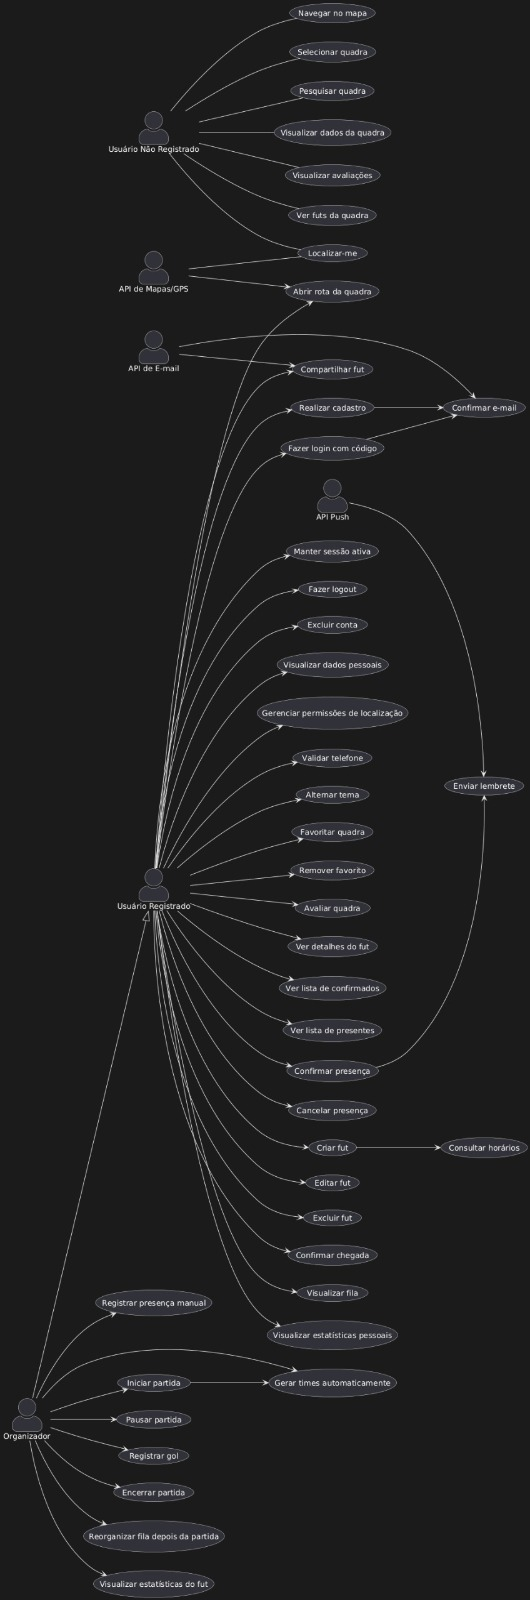
\includegraphics[width=\linewidth]{figuras/uc-borafut.png}
      \caption{Diagrama de casos de uso do \textbf{BoraFut} (gerado no Lucid).}
      \label{fig:uc-borafut}
      \end{figure}

  \section{Fluxos principais}
    Os fluxos de uso representam a sequência de ações realizadas pelos usuários dentro do aplicativo para alcançar seus objetivos. Cada fluxo descreve o caminho percorrido desde a intenção inicial até a conclusão da tarefa, garantindo que as interações do sistema sejam coerentes, intuitivas e acessíveis. A seguir, são descritos os principais fluxos que compõem o escopo do MVP.

    \subsection{Criar conta}
      O processo de criação de conta segue o modelo de autenticação \textit{passwordless}, baseado exclusivamente no e-mail do usuário. Ao abrir o aplicativo pela primeira vez, o usuário informa seu endereço de e-mail em um único campo. O sistema envia um código temporário para o e-mail informado e, ao retornar ao aplicativo, o usuário insere esse código para prosseguir.

      Se o e-mail ainda não estiver associado a uma conta, o usuário é direcionado para a etapa de cadastro, onde preenche informações básicas como nome, apelido e, opcionalmente, posição preferida em quadra. Após concluir essa etapa, sua conta é criada e o acesso às funcionalidades do aplicativo é liberado. Caso o e-mail já esteja registrado, o usuário é autenticado diretamente após a verificação do código.

    \subsection{Fazer login}
      Para autenticar-se, o usuário informa seu e-mail registrado e recebe um código temporário enviado automaticamente. Ao inserir o código corretamente, o sistema valida sua identidade e inicia a sessão. A autenticação não utiliza senhas, reduzindo atritos de acesso e eliminando riscos associados ao armazenamento local de credenciais. Uma vez autenticado, o usuário permanece logado até encerrar manualmente a sessão.

    \subsection{Visualizar quadras}
    Ao entrar no aplicativo, o usuário é direcionado ao mapa interativo, centralizado em sua localização atual. As quadras próximas são exibidas como marcadores, permitindo navegação, zoom e movimentação livre no mapa. O usuário pode buscar quadras pelo nome, aplicar filtros e selecionar qualquer marcador para visualizar informações detalhadas sobre a quadra escolhida.

    \subsection{Visualizar perfil da quadra}
    Ao selecionar um marcador no mapa, o usuário acessa o perfil da quadra, onde encontra informações como endereço, características básicas, avaliação média, futs recentes e futs agendados. A tela apresenta também o botão “Como chegar”, que abre o aplicativo de mapas do dispositivo com rota até o local. Usuários autenticados podem favoritar a quadra para acessá-la rapidamente no futuro.

    \subsection{Visualizar agenda da quadra}
    No perfil de uma quadra, o usuário pode consultar futs agendados e eventos recorrentes para os próximos dias. Essa agenda auxilia na escolha de horários disponíveis e fornece uma noção da atividade da quadra ao longo da semana.

    \subsection{Criar fut}
    Após selecionar uma quadra, o usuário autenticado pode criar um fut clicando no botão correspondente. O sistema exibe um formulário solicitando data, horário, modalidade e uma descrição opcional. Ao confirmar, o fut é registrado e passa a estar disponível para visualização no perfil da quadra e no mapa para outros usuários.

    \subsection{Visualizar fut e confirmar presença}
    Ao explorar o mapa ou o perfil da quadra, o usuário pode selecionar um fut específico. A tela apresenta informações completas, incluindo horário, vagas disponíveis e regras básicas. Usuários autenticados podem confirmar ou cancelar presença com um toque. A confirmação atualiza imediatamente o total de jogadores e a ordem de chegada virtual.

    \subsection{Enviar convite}
    Jogadores que já confirmaram presença em uma partida podem convidar outras pessoas para participar. A partir da tela do fut, o usuário clica em “Enviar convite” e escolhe o aplicativo de sua preferência (como WhatsApp ou Telegram) para compartilhar um link direto para o jogo. Ao clicar no link, o convidado é redirecionado ao aplicativo e pode confirmar presença com poucos toques.

    \subsection{Confirmar chegada}
    No horário do fut, o usuário acessa a tela da partida e seleciona a opção “Confirmar chegada”. O botão fica disponível apenas a partir do horário agendado do fut. O registro de chegada atualiza a ordem da fila de jogadores, permitindo que o sistema gere times iniciais e organize futuras rotações. A confirmação é manual, mas pode ser apoiada por verificação de localização, desde que o usuário esteja próximo à quadra.

    \subsection{Iniciar o fut}
      O criador do fut tem a permissão para iniciar a partida assim que o horário agendado é alcançado. Ele pode acessar rapidamente o perfil da partida por meio do \textit{popup} de destaque e iniciar o jogo, fazendo com que o sistema gere automaticamente os dois times iniciais com base na ordem de chegada e organize os próximos times na fila. Jogadores que chegarem após o início são posicionados no final da lista.

    \subsection{Gerenciar fut}
    Durante a partida, os jogadores em espera tem acesso aos controles de jogo, incluindo pausar e retomar o cronômetro, registrar gols e encerrar a partida. Ao finalizar, o sistema atualiza automaticamente a fila de jogadores conforme as regras definidas e registra dados básicos, como placar e jogadores presentes. Esses dados são utilizados para gerar estatísticas simples do fut e dos participantes.

    \subsection{Cadastro manual de jogadores}
    Nem todos os participantes possuem aplicativo, internet ou conta ativa. Para esses casos, o sistema permite o cadastro manual. Um jogador já logado pode abrir o perfil do fut e clicar em “Adicionar participante manualmente”, preenchendo nome e e-mail do colega. Dessa forma, mesmo sem conexão, o jogador é incluído oficialmente na partida.

    \subsection{Rota para a quadra}
    Para facilitar o deslocamento até o local do jogo, o aplicativo disponibiliza um botão “Como chegar” em cada perfil de quadra. Ao ser acionado, o sistema gera um \textit{deep link} que abre automaticamente o aplicativo de mapas padrão do dispositivo com a rota traçada até o endereço da quadra, facilitando o deslocamento até o local do fut.

  \section{Design de interface REVISAR E REFAZER}
    O design de interface do \textbf{BoraFut} reflete a identidade visual definida no documento interno
    \textit{Borafut — Manual de Identidade Visual}~\cite{borafut_visual2025}, desenvolvido pela equipe do projeto.
    Esse guia estabelece os elementos fundamentais da marca, como paleta de cores, tipografia, ícones e
    diretrizes de uso, garantindo unidade estética e coerência entre o aplicativo e suas demais comunicações.

    \subsection{Identidade visual}
      A identidade visual foi concebida para transmitir energia, simplicidade e senso de comunidade,
      valores centrais do \textbf{BoraFut}. A marca utiliza proporções uniformes e formas geométricas simples,
      reforçando o equilíbrio e a clareza visual. O logotipo adota uma fonte monoespaçada de traços arredondados,
      inspirada na tipografia \textit{Dune Rise}, de Jesta Designs, ajustada para criar uma sensação mais próxima e
      acolhedora ao contexto esportivo e comunitário.

      A paleta principal é composta por tons de ciano, que simbolizam vitalidade, confiança e dinamismo,
      complementados por cinza e branco, que equilibram e conferem sofisticação à composição visual.
      Essas cores aparecem de forma consistente na interface do aplicativo, desde os botões até os
      elementos de navegação, reforçando o reconhecimento da marca.

      A tipografia escolhida para a interface é a \textbf{Open Sans}, uma fonte sem serifa amplamente usada em
      ambientes digitais. Sua legibilidade em diferentes tamanhos de tela e sua aparência moderna contribuem
      para uma leitura agradável e fluida. Essa combinação de tipografia e cores cria uma experiência visual
      que equilibra leveza e clareza, tornando a navegação mais intuitiva para o usuário.

    \subsection{Diretrizes de acessibilidade}
      O design do aplicativo foi desenvolvido com base em princípios de acessibilidade digital, garantindo que
      o \textbf{BoraFut} possa ser utilizado por públicos diversos, independentemente de idade ou familiaridade
      com tecnologia. As diretrizes seguem recomendações das \textit{Web Content Accessibility Guidelines} (WCAG~2.1),
      incluindo contraste mínimo de 4.5:1 entre texto e fundo, botões com dimensões adequadas ao toque (mínimo
      de 44x44~px) e ícones acompanhados de rótulos descritivos. 

      O layout foi projetado para oferecer hierarquia visual clara, com espaçamentos amplos e elementos
      interativos bem destacados. O aplicativo também suporta modo escuro, reduzindo o cansaço visual em
      uso prolongado, e utiliza linguagem neutra e inclusiva em suas mensagens e labels.

    \subsection{Heurísticas de Nielsen e usabilidade}
      As decisões de design foram orientadas pelos princípios heurísticos de usabilidade propostos por
      Jakob Nielsen~(1994), amplamente reconhecidos na área de Interação Humano-Computador. Entre os
      aplicados ao \textbf{BoraFut}, destacam-se:

      \begin{itemize}
          \item \textbf{Visibilidade do status do sistema}: o usuário recebe feedback imediato ao confirmar presença,
          criar um jogo ou realizar qualquer ação relevante, por meio de mensagens e animações sutis;
          \item \textbf{Correspondência entre o sistema e o mundo real}: o aplicativo utiliza termos próximos da
          linguagem cotidiana dos jogadores, como “fut”, “bora jogar” e “confirmar presença”;
          \item \textbf{Controle e liberdade do usuário}: o usuário pode editar, cancelar ou sair de ações a qualquer
          momento, evitando erros permanentes;
          \item \textbf{Consistência e padrões}: ícones, botões e cores seguem padrões estáveis, reduzindo a curva
          de aprendizado e promovendo previsibilidade;
          \item \textbf{Prevenção e recuperação de erros}: as mensagens de erro são claras e instrutivas, indicando o
          que deve ser feito para corrigir o problema.
      \end{itemize}

      Essas diretrizes asseguram uma interface coerente, acessível e orientada à experiência do usuário,
      favorecendo o engajamento e reduzindo barreiras de uso para diferentes perfis de jogadores.

  \section{Prototipação}
  \section{Arquitetura e design}
    \label{sec:arquitetura-design}

    Esta seção apresenta a arquitetura técnica e a modelagem do banco de dados do \textit{BORAFUT}, descrevendo como as decisões planejadas na metodologia (Seção~\ref{sec:arquitetura-geral}) foram concretizadas em artefatos. São exibidos dois diagramas baseados no modelo C4, que representam a estrutura do sistema em diferentes níveis de abstração, seguidos do modelo de dados do banco \textit{PostgreSQL}.

    \subsection{Modelo C4 de contexto e contêineres}
      \label{subsec:c4}

      O modelo C4, proposto por Brown~\cite{brown2018}, é um método visual para documentar arquitetura de software em quatro níveis de abstração: contexto, contêineres, componentes e código, que permitem descrever a arquitetura de software em diferentes graus de detalhe. 
      Neste trabalho, optou-se por representar apenas os dois primeiros níveis (contexto e contêineres), por serem suficientes para comunicar a visão geral e a organização técnica do \textit{BORAFUT} no estágio atual do projeto. 

      \subsubsection{Diagrama de contexto (C1).}
        O diagrama de contexto mostra o \textit{BORAFUT} como um sistema inserido em seu ambiente de uso. Ele representa as interações entre os usuários e os sistemas externos que fornecem serviços complementares.  
        Na Figura~\ref{fig:c4-contexto}, observa-se que o aplicativo é utilizado por jogadores amadores e administradores de quadra, comunicando-se com serviços responsáveis por autenticação e geolocalização.

        \begin{figure}[h]
            \centering
            % 
\includegraphics[width=0.8\textwidth]{figures/c4-contexto.png}
            \caption{Diagrama C4 nível contexto do \textit{BORAFUT}.}
            \label{fig:c4-contexto}
        \end{figure}

      \subsubsection{Diagrama de contêineres (C2).}
        O diagrama de contêineres representa a decomposição interna do sistema em suas principais partes executáveis, chamadas de contêineres. Cada contêiner abriga um conjunto de responsabilidades técnicas ou funcionais, comunicando-se com os demais por interfaces bem definidas.  

        A Figura~\ref{fig:c4-conteineres} apresenta os principais contêineres do \textit{BORAFUT}:
        \begin{itemize}
            \item o \textbf{aplicativo móvel} (\textit{React Native}), responsável pela interação com o usuário e envio das requisições à API;
            \item o \textbf{backend} (\textit{Node.js + Express}), que concentra a lógica de negócio, autenticação e orquestração de dados;
            \item o \textbf{banco de dados relacional} (\textit{PostgreSQL}), que armazena as informações persistentes;
            \item e as \textbf{APIs externas}, usadas para autenticação (\textit{Google Identity}), geolocalização (\textit{Google Maps Platform}) e armazenamento de mídia.
        \end{itemize}

        \begin{figure}[h]
            \centering
            % 
\includegraphics[width=0.8\textwidth]{figures/c4-conteineres.png}
            \caption{Diagrama C4 nível contêineres do \textit{BORAFUT}.}
            \label{fig:c4-conteineres}
        \end{figure}

    \subsection{Modelo de dados do PostgreSQL}
      \label{subsec:modelo-dados}

      O modelo de dados do \textit{BORAFUT} foi elaborado com base nas entidades e relacionamentos identificados durante o levantamento de requisitos (Capítulo~\ref{sec:metodologia-elicitacao}). O objetivo é garantir que as informações essenciais, como jogadores, partidas e quadras sejam armazenadas de forma estruturada, mantendo a integridade referencial.

      A modelagem seguiu uma abordagem relacional normalizada, organizada em tabelas interconectadas por chaves primárias e estrangeiras. Entre as principais entidades estão:
      
      \begin{itemize}
          \item \textbf{Jogador} — dados pessoais, preferências e histórico de partidas;
          \item \textbf{Quadra} — informações sobre localização, disponibilidade e avaliações;
          \item \textbf{Partida} — definição de horários, participantes e status;
      \end{itemize}

      A Figura~\ref{fig:modelo-dados} apresenta o modelo entidade-relacionamento (MER) que representa o modelo lógico do banco de dados planejado.

      \begin{figure}[h]
          \centering
          % 
\includegraphics[width=0.9\textwidth]{figures/modelo-dados.png}
          \caption{Modelo entidade-relacionamento do banco \textit{PostgreSQL}.}
          \label{fig:modelo-dados}
      \end{figure}

      O modelo entidade–relacionamento completo encontra-se no Apêndice \ref{apendice:MER} que apresenta o modelo lógico do banco de dados.

    % \subsection{Contratos de API REST}
    % Endpoints, métodos e esquemas
    
    % \subsection{Decisões arquiteturais registradas em ADRs curtas}

    % \section{Teste de usabilidade}
    % Descrever o teste conduzido para validação do MVP
    % Incluir público participante, cenários de uso, métricas e resultados observados
    % Sumário de ADRs

  \section{Prova de conceito}
    % Demonstração mínima: mapa com pins da API Express; ação de abrir rota por deep link; prints e repositório


